\documentclass[10pt,a4paper]{article}
\usepackage[a4paper,margin=16mm,top=15mm,bottom=16mm,columnsep=7mm]{geometry}
\usepackage[T1]{fontenc}
\usepackage[utf8]{inputenc}
\usepackage{newtxtext,newtxmath}
\usepackage{microtype}
\usepackage{booktabs}
\usepackage{tabularx}
\usepackage{array}
\usepackage{enumitem}
\usepackage{tikz}
\usetikzlibrary{arrows.meta,positioning,fit,calc,backgrounds}
\usepackage[most]{tcolorbox}
\usepackage{titlesec}
\usepackage{xcolor}
\usepackage[hidelinks]{hyperref}
\usepackage{fancyhdr}
\usepackage{parskip}
\usepackage{ragged2e}
\usepackage{multicol}
\usepackage{amsmath}
\usepackage{listings}

\definecolor{ink}{HTML}{17202A}
\definecolor{muted}{HTML}{566573}
\definecolor{navy}{HTML}{183A59}
\definecolor{blue}{HTML}{2E75B6}
\definecolor{teal}{HTML}{168A8A}
\definecolor{green}{HTML}{2E7D5B}
\definecolor{amber}{HTML}{B87900}
\definecolor{violet}{HTML}{6A4C93}
\definecolor{rose}{HTML}{A83F5F}
\definecolor{panel}{HTML}{F5F7FA}
\definecolor{line}{HTML}{D7DEE5}

\setlength{\parindent}{0pt}
\setlist[itemize]{leftmargin=1.2em,itemsep=1pt,topsep=2pt,label=\textcolor{blue}{\scriptsize\textbullet}}
\setlist[enumerate]{leftmargin=1.4em,itemsep=1pt,topsep=2pt}
\renewcommand{\arraystretch}{1.05}
\setlength{\tabcolsep}{3.5pt}
\setlength{\emergencystretch}{2.5em}

\titleformat{\section}{\large\bfseries\color{navy}}{}{0pt}{}
\titleformat{\subsection}{\normalsize\bfseries\color{ink}}{}{0pt}{}
\titlespacing*{\section}{0pt}{7pt}{3pt}
\titlespacing*{\subsection}{0pt}{5pt}{2pt}

\pagestyle{fancy}
\fancyhf{}
\fancyhead[L]{\footnotesize\textcolor{muted}{UMLCAD.V.7}}
\fancyhead[R]{\footnotesize\textcolor{muted}{.NET Library Architecture Reference}}
\fancyfoot[C]{\footnotesize\textcolor{muted}{\thepage}}
\renewcommand{\headrulewidth}{0.35pt}
\renewcommand{\footrulewidth}{0pt}

\newcommand{\code}[1]{\texttt{\footnotesize #1}}
\newcommand{\filepath}[1]{\path{#1}}

\newtcolorbox{infobox}{
 enhanced,colback=panel,colframe=line,boxrule=0.5pt,arc=2mm,
 left=5pt,right=5pt,top=4pt,bottom=4pt,before skip=4pt,after skip=5pt}

\newtcolorbox{authoritybox}{
 enhanced,colback=navy!4,colframe=navy!45,boxrule=0.7pt,arc=2mm,
 left=6pt,right=6pt,top=5pt,bottom=5pt,before skip=4pt,after skip=5pt}

\lstset{basicstyle=\ttfamily\scriptsize,breaklines=true,columns=fullflexible,keepspaces=true,frame=none}

\tikzset{
 lib/.style={draw,rounded corners=2pt,very thick,minimum width=4.1cm,minimum height=1.05cm,align=left,inner sep=6pt,font=\sffamily\scriptsize},
 app/.style={lib,fill=blue!8,draw=blue!60!black},
 cad/.style={lib,fill=teal!8,draw=teal!60!black},
 eng/.style={lib,fill=green!8,draw=green!55!black},
 sci/.style={lib,fill=violet!8,draw=violet!60!black},
 kernel/.style={lib,fill=rose!7,draw=rose!60!black},
 contract/.style={lib,fill=amber!8,draw=amber!65!black},
 arr/.style={-{Latex[length=2.4mm]},line width=0.75pt,draw=muted!80},
 arr2/.style={-{Latex[length=2.4mm]},line width=0.55pt,draw=line!100}}

\begin{document}

\begin{center}
{\sffamily\bfseries\fontsize{20}{22}\selectfont\color{navy}UMLCAD.V.7}\par
\vspace{1mm}
{\sffamily\bfseries\fontsize{13}{15}\selectfont\color{ink}Current .NET Library Architecture and Class Map}\par
\vspace{1mm}
{\sffamily\small\color{muted}Main branch baseline: \code{ccdf4a6b7122d945456432a91cfc7398fa1f9738}\quad|\quad 12 production libraries}\par
\vspace{5mm}

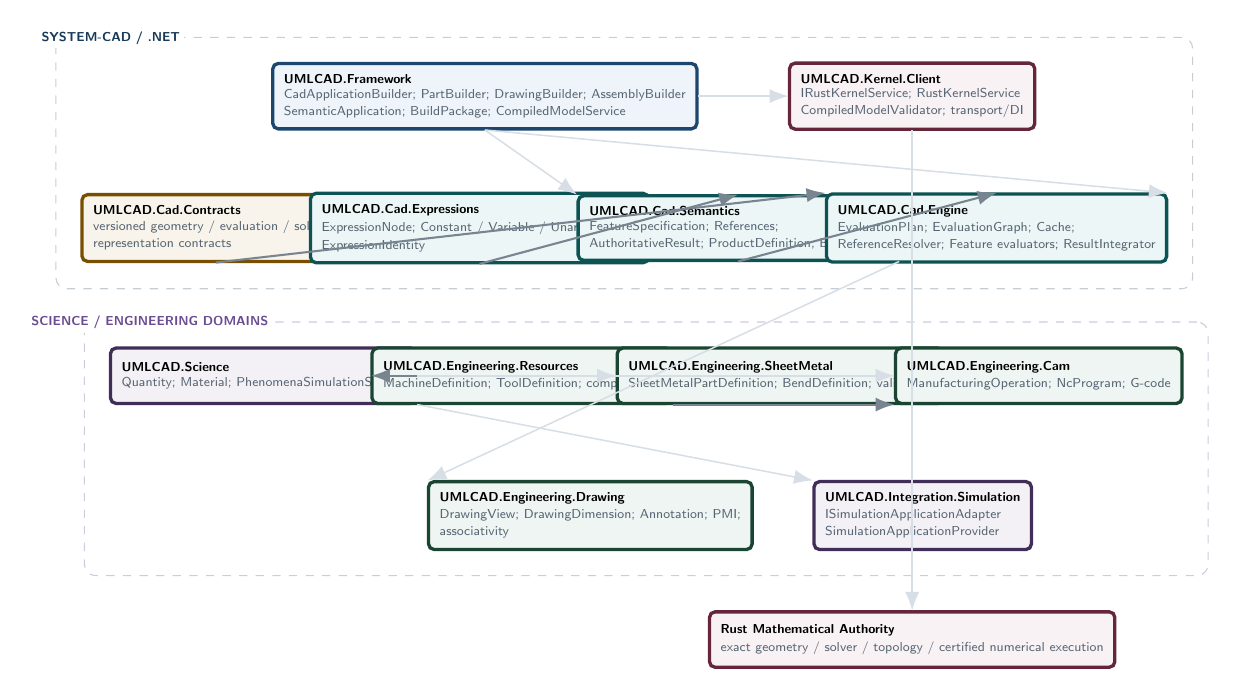
\begin{tikzpicture}[x=1cm,y=1cm,scale=0.67,transform shape]
\node[app] (framework) at (0,5.3) {\shortstack[l]{\textbf{UMLCAD.Framework}\\\textcolor{muted}{CadApplicationBuilder; PartBuilder; DrawingBuilder; AssemblyBuilder}\\\textcolor{muted}{SemanticApplication; BuildPackage; CompiledModelService}}};
\node[kernel] (kclient) at (8.1,5.3) {\shortstack[l]{\textbf{UMLCAD.Kernel.Client}\\\textcolor{muted}{IRustKernelService; RustKernelService}\\\textcolor{muted}{CompiledModelValidator; transport/DI}}};

\node[contract] (contracts) at (-5.1,2.8) {\shortstack[l]{\textbf{UMLCAD.Cad.Contracts}\\\textcolor{muted}{versioned geometry / evaluation / solver /}\\\textcolor{muted}{representation contracts}}};
\node[cad] (expr) at (-0.1,2.8) {\shortstack[l]{\textbf{UMLCAD.Cad.Expressions}\\\textcolor{muted}{ExpressionNode; Constant / Variable / Unary / Binary}\\\textcolor{muted}{ExpressionIdentity}}};
\node[cad] (sem) at (4.8,2.8) {\shortstack[l]{\textbf{UMLCAD.Cad.Semantics}\\\textcolor{muted}{FeatureSpecification; References;}\\\textcolor{muted}{AuthoritativeResult; ProductDefinition; BomService}}};
\node[cad] (engine) at (9.7,2.8) {\shortstack[l]{\textbf{UMLCAD.Cad.Engine}\\\textcolor{muted}{EvaluationPlan; EvaluationGraph; Cache;}\\\textcolor{muted}{ReferenceResolver; Feature evaluators; ResultIntegrator}}};

\node[sci] (science) at (-4.2,0.0) {\shortstack[l]{\textbf{UMLCAD.Science}\\\textcolor{muted}{Quantity; Material; PhenomenaSimulationService}}};
\node[eng] (resources) at (0.7,0.0) {\shortstack[l]{\textbf{UMLCAD.Engineering.Resources}\\\textcolor{muted}{MachineDefinition; ToolDefinition; compatibility}}};
\node[eng] (sheet) at (5.6,0.0) {\shortstack[l]{\textbf{UMLCAD.Engineering.SheetMetal}\\\textcolor{muted}{SheetMetalPartDefinition; BendDefinition; validation}}};
\node[eng] (cam) at (10.5,0.0) {\shortstack[l]{\textbf{UMLCAD.Engineering.Cam}\\\textcolor{muted}{ManufacturingOperation; NcProgram; G-code}}};

\node[eng] (drawing) at (2.0,-2.65) {\shortstack[l]{\textbf{UMLCAD.Engineering.Drawing}\\\textcolor{muted}{DrawingView; DrawingDimension; Annotation; PMI;}\\\textcolor{muted}{associativity}}};
\node[sci] (sim) at (8.3,-2.65) {\shortstack[l]{\textbf{UMLCAD.Integration.Simulation}\\\textcolor{muted}{ISimulationApplicationAdapter}\\\textcolor{muted}{SimulationApplicationProvider}}};
\node[kernel,minimum width=5.2cm] (rust) at (8.1,-5.0) {\shortstack[l]{\textbf{Rust Mathematical Authority}\\\textcolor{muted}{exact geometry / solver / topology / certified numerical execution}}};

\draw[arr] (expr.south) -- (sem.north);
\draw[arr] (sem.south) -- (engine.north);
\draw[arr] (contracts.south) -- (engine.north west);
\draw[arr2] (framework.south) -- (sem.north west);
\draw[arr2] (framework.south) -- (engine.north east);
\draw[arr2] (framework.east) -- (kclient.west);
\draw[arr] (science.east) -- (resources.west);
\draw[arr2] (science.east) -- (sheet.west);
\draw[arr2] (science.east) -- (cam.west);
\draw[arr2] (sem.south east) -- (drawing.north west);
\draw[arr2] (science.south east) -- (sim.north west);
\draw[arr] (resources.south east) -- (cam.south west);
\draw[arr2] (kclient.south) -- (rust.north);

\begin{scope}[on background layer]
\node[draw=navy!25,dashed,rounded corners=4pt,fit=(framework)(contracts)(expr)(sem)(engine),inner sep=9pt] (cadframe) {};
\node[fill=white,inner sep=2pt,font=\sffamily\scriptsize\bfseries\color{navy}] at ($(cadframe.north west)+(1.05,-0.02)$) {SYSTEM-CAD / .NET};
\node[draw=violet!30,dashed,rounded corners=4pt,fit=(science)(resources)(sheet)(cam)(drawing)(sim),inner sep=9pt] (engframe) {};
\node[fill=white,inner sep=2pt,font=\sffamily\scriptsize\bfseries\color{violet}] at ($(engframe.north west)+(1.25,-0.02)$) {SCIENCE / ENGINEERING DOMAINS};
\end{scope}
\end{tikzpicture}

\vspace{2mm}
\begin{infobox}
\centering\small
\textbf{Authority rule:} .NET libraries own semantic meaning, contracts, orchestration and engineering-domain logic. The existing Rust kernel remains the mathematical authority. The engineering-library merge changed neither \code{kernel/**} nor the existing \code{UMLCAD.Kernel.Client} source.
\end{infobox}
\end{center}

\begin{multicols}{2}
\raggedcolumns

\section{Document scope and current baseline}
This reference describes the production .NET libraries actually present under \filepath{dotnet/src/} on the current \code{main} branch. Every library has a project boundary, source inventory, dependency statement, ownership rule and current capability boundary.

\begin{authoritybox}
\textbf{Baseline.} Final engineering-library merge commit: \code{ccdf4a6b7122d945456432a91cfc7398fa1f9738}. The post-merge comparison against the pre-merge main commit reported zero changes under \code{kernel/**} and zero changes under \code{dotnet/src/UMLCAD.Kernel.Client/**}.
\end{authoritybox}

\section{Global .NET conventions}
All production libraries target \code{net10.0}, enable nullable reference types and implicit usings, and treat warnings as errors. The SDK is pinned by \filepath{dotnet/global.json}.

The semantic/domain model is record-first and immutable where practical. Identity-bearing serialization is deterministic. Invalid or uncertain states are preserved explicitly instead of being silently repaired.

\subsection{Authority split}
\begin{itemize}
\item \textbf{Semantics} owns engineering intent.
\item \textbf{Evaluation} owns execution orchestration.
\item \textbf{Contracts} own stable provider boundaries.
\item \textbf{Engineering domains} own domain-specific semantics and workflows.
\item \textbf{Kernel Client} owns transport.
\item \textbf{Rust} remains mathematical authority.
\end{itemize}

\section{Library landscape}
\small
\begin{tabularx}{\columnwidth}{@{}>{\raggedright\arraybackslash}p{0.38\columnwidth}X@{}}
\toprule
Library & Primary responsibility\\
\midrule
\filepath{UMLCAD.Framework} & Application composition, authoring, semantic snapshot, build identity/history, package and compiled semantic graph.\\
\filepath{UMLCAD.Kernel.Client} & Existing .NET-to-Rust build/evaluation transport and result-integrity boundary.\\
\filepath{UMLCAD.Cad.Contracts} & Versioned CAD, geometry, solver and representation contracts.\\
\filepath{UMLCAD.Cad.Expressions} & Pure arithmetic expressions and deterministic expression identity.\\
\filepath{UMLCAD.Cad.Semantics} & Feature semantics, references, authoritative results, product structure/BOM.\\
\filepath{UMLCAD.Cad.Engine} & Evaluation graph/planning, invalidation, caching, reference resolution and result integration.\\
\filepath{UMLCAD.Science} & Quantities, dimensions, materials and phenomena simulation contracts.\\
\filepath{UMLCAD.Engineering.Resources} & Machines, tools, processes, capabilities and compatibility.\\
\filepath{UMLCAD.Engineering.SheetMetal} & Sheet-metal semantics, bend expressions and validation.\\
\filepath{UMLCAD.Engineering.Cam} & Manufacturing operations, toolpaths, postprocessing and deterministic NC/G-code.\\
\filepath{UMLCAD.Engineering.Drawing} & Views, dimensions, annotations, dress-up, PMI, BOM presentation and associativity.\\
\filepath{UMLCAD.Integration.Simulation} & External simulation application adapters.\\
\bottomrule
\end{tabularx}
\normalsize

\section{UMLCAD.Cad.Contracts}
\textbf{Project:} \filepath{dotnet/src/UMLCAD.Cad.Contracts/}\\
\textbf{Dependencies:} none.

\textbf{Source files:} \code{AxisAlignedBoxSolidContracts.cs}, \code{CadEvaluationContracts.cs}, \code{CircularPrismSolidContracts.cs}, \code{ExtrusionContracts.cs}, \code{GeometryKernelStatus.cs}, \code{KernelContracts.cs}, \code{RepresentationContracts.cs}, \code{SketchSolveContracts.cs}.

\subsection{Principal contract families}
\begin{itemize}
\item \code{CadId}, \code{CadResultId}, \code{TopologyEntityId}: explicit identity values.
\item \code{CadFrame}, \code{CadVector3}, \code{CadBoundingBox3}: coordinate/result contracts. Frames validate finite origin, orthonormal basis and right-handed orientation.
\item \code{ReferenceContext}, \code{TopologySelector}, \code{CadReference}, \code{ReferenceResolution}: explicit reference semantics.
\item Axis-aligned box, circular-prism and convex-planar-extrusion request/result contracts define narrow authoritative operations.
\item \code{SketchSolveRequest}, \code{SketchSolveKernelResult}, \code{ISketchConstraintService}: bounded sketch-solver boundary.
\item Generic kernel/representation envelopes preserve contract version, operation identity, result identity and evidence.
\end{itemize}

\begin{infobox}\small
Contracts are boundaries, not algorithms. They must remain independent from a concrete mathematical implementation.
\end{infobox}

\section{UMLCAD.Cad.Expressions}
\textbf{Project:} \filepath{dotnet/src/UMLCAD.Cad.Expressions/}\\
\textbf{Dependencies:} none.

\textbf{Source files:} \code{ArithmeticExpression.cs}, \code{ExpressionIdentity.cs}.

\subsection{Class family}
\code{ExpressionNode} is the immutable root. Current forms are \code{ConstantExpression}, \code{VariableExpression}, \code{UnaryExpression} and \code{BinaryExpression}. Nodes support numerical evaluation and canonical serialization.

\code{ExpressionIdentity} derives SHA-256 identity from canonical expression structure. Runtime object identity, timestamps and rendering state are excluded.

\section{UMLCAD.Cad.Semantics}
\textbf{Project:} \filepath{dotnet/src/UMLCAD.Cad.Semantics/}\\
\textbf{Dependencies:} \code{UMLCAD.Cad.Expressions}.

\textbf{Source files:} \code{AuthoritativeResults.cs}, \code{FeatureSpecifications.cs}, \code{ProductStructure.cs}, \code{References.cs}.

\subsection{Feature semantics}
Immutable feature intent includes the current bounded box, sketch/profile and extrusion structures. These definitions are semantic intent and are not kernel geometry objects.

\subsection{Reference semantics}
Current concepts include \code{ReferenceTargetKind}, \code{ReferenceResolutionStatus}, \code{ReferenceContextId}, \code{ReferencePathSegment}, \code{ReferencePath}, \code{CadReference}, \code{SemanticReference}, \code{GeometricReference}, \code{TopologyReference}, \code{ReferenceResolution} and \code{TopologyEvolution}. Evolution distinguishes preserved, replaced, split, merged, removed, introduced and ambiguous topology.

\subsection{Authoritative results}
\code{AuthoritativeResultIdentity}, \code{AuthoritativeResultKind}, \code{AuthoritativeResultStatus}, \code{TopologyBinding}, \code{ResultEvidence} and \code{AuthoritativeCadResult} represent certified-result meaning separately from derived representations.

\subsection{Product structure and BOM}
\code{SemanticId}, \code{ProductComponent}, \code{ProductOccurrence}, \code{ProductDefinition}, \code{BomLine} and \code{BomService} define reusable component definitions and contextual occurrences. BOM grouping, aggregation and ordering are deterministic.

\section{UMLCAD.Cad.Engine}
\textbf{Project:} \filepath{dotnet/src/UMLCAD.Cad.Engine/}\\
\textbf{Dependencies:} Expressions, Semantics, Contracts.

\textbf{Source files:} \code{AsyncEvaluationEngine.cs}, \code{AuthoritativeCadReferenceResolver.cs}, \code{AxisAlignedBoxSolidEvaluator.cs}, \code{CadEvaluationEngine.cs}, \code{CadModelEvaluator.cs}, \code{ChangeSets.cs}, \code{ConvexProfileExtrusionEvaluator.cs}, \code{EvaluationCache.cs}, \code{EvaluationEngine.cs}, \code{EvaluationGraph.cs}, \code{EvaluationIdentityBuilder.cs}, \code{EvaluationStepFactory.cs}, \code{FeatureEvaluation.cs}, \code{IncrementalEvaluation.cs}, \code{ReferenceResolver.cs}, \code{ResultIntegration.cs}.

\subsection{Evaluation graph}
The Engine separates specification, execution and result graphs. \code{EvaluationStep}, \code{EvaluationPlan} and \code{EvaluationGraph} encode deterministic dependency order. Cycles and unresolved dependencies fail explicitly.

\subsection{Evaluation identity and cache}
\code{EvaluationIdentityBuilder} hashes operation, normalized definition, dependencies, input identities, configuration, tolerance, kernel contract and representation policy. \code{EvaluationCache} stores results by evaluation identity.

\subsection{Incremental recomputation}
\code{CadChangeSet}, \code{IncrementalEvaluationPlan} and \code{IncrementalEvaluationPlanner} calculate affected closures. Incremental execution is an optimization of one semantic function, not a second semantics.

\subsection{Reference resolution and execution}
\code{ReferenceResolver} and \code{AuthoritativeCadReferenceResolver} resolve semantic, result and topology references. \code{AxisAlignedBoxSolidEvaluator} and \code{ConvexProfileExtrusionEvaluator} adapt bounded authoritative operations into contracts. Exact B-Rep mathematics remains outside this library.

\section{UMLCAD.Science}
\textbf{Project:} \filepath{dotnet/src/UMLCAD.Science/}\\
\textbf{Dependencies:} Expressions.

\textbf{Source files:} \code{PhenomenaSimulationService.cs}, \code{ScienceFoundation.cs}.

\subsection{Core classes}
\code{QuantityDimension} models dimensional powers. \code{Quantity} stores SI value, dimensional signature and unit symbol. \code{MaterialFamily}, \code{MaterialProperties} and \code{Material} provide shared scientific/material semantics.

\code{PhenomenonKind}, \code{PhenomenaSimulationRequest}, \code{PhenomenaSimulationResult}, \code{IPhenomenaSimulationProvider}, \code{IPhenomenaSimulationService} and \code{PhenomenaSimulationService} define provider-neutral phenomena simulation.

This library defines the simulation boundary; it is not itself a general physics solver.

\section{UMLCAD.Engineering.Resources}
\textbf{Project:} \filepath{dotnet/src/UMLCAD.Engineering.Resources/}\\
\textbf{Dependencies:} Expressions, Science.

\textbf{Source file:} \code{EngineeringResources.cs}.

\subsection{Resource model}
\code{MachineKind}, \code{ToolKind} and \code{ManufacturingProcessKind} define the current vocabulary. \code{MachineCapability} models process/thickness capability. \code{ToolDefinition} models tool identity, interface and diameter constraints. \code{MachineDefinition} aggregates machine capabilities.

\code{MachineProcessCompatibility}, \code{ToolProcessCompatibility} and \code{MachineToolCompatibility} implement fail-closed compatibility rules.

\section{UMLCAD.Engineering.SheetMetal}
\textbf{Project:} \filepath{dotnet/src/UMLCAD.Engineering.SheetMetal/}\\
\textbf{Dependencies:} Expressions, Semantics, Science, Resources.

\textbf{Source files:} \code{SheetMetalExpressions.cs}, \code{SheetMetalSemantics.cs}.

\subsection{Semantic classes}
\code{SheetMetalPartDefinition}, \code{BendDefinition}, \code{SheetMetalValidationResult} and \code{SheetMetalValidator} connect material, thickness, ductility, bend geometry and manufacturing feasibility.

The bend allowance is represented using the shared expression AST:
\[
\left(\frac{\pi}{180}\right)(R+KT)A.
\]

The current library is a sheet-metal semantic/manufacturing foundation, not a complete exact folding/unfolding B-Rep engine.

\section{UMLCAD.Engineering.Cam}
\textbf{Project:} \filepath{dotnet/src/UMLCAD.Engineering.Cam/}\\
\textbf{Dependencies:} Expressions, Semantics, Science, Resources.

\textbf{Source file:} \code{CamAndGCode.cs}.

\subsection{CAM class family}
\code{ToolpathPoint} stores finite XYZ motion points. \code{ManufacturingOperation} stores operation identity, process, tool, stock thickness and ordered path. \code{NcProgram} stores program/machine identity and deterministic lines, with \code{Serialize()} and \code{ContentHash()}.

\code{INcPostprocessor} is the postprocessor boundary. \code{DeterministicGCodePostprocessor} currently emits bounded milling G-code after resource compatibility checks. \code{CamPhenomenaAdvisor} uses Science phenomena services.

CAM does not create mathematical CAD truth. The intended chain is authoritative CAD result -> manufacturing planning -> toolpath -> resource validation -> postprocessor -> NC/G-code.

\section{UMLCAD.Engineering.Drawing}
\textbf{Project:} \filepath{dotnet/src/UMLCAD.Engineering.Drawing/}\\
\textbf{Dependencies:} Expressions, Semantics, Science.

\textbf{Source files:} \code{DrawingSemantics.cs}, \code{DrawingAdvancedSemantics.cs}.

\subsection{Drawing vocabulary}
Current semantics cover ISO/ANSI/JIS standards, orthographic/isometric/auxiliary/section/detail/clipping/broken/unfolded view families, linear/angular/radius/diameter/coordinate/baseline/chain dimensions, annotation types including datum/GD\&T/surface roughness/welding, and dress-up concepts.

\subsection{Principal classes}
\code{DrawingSheet}, \code{DrawingView}, \code{DrawingDimension}, \code{DrawingAnnotation}, \code{DrawingCapabilityMatrix}, \code{MechanicalDraftingCapabilityProfile}, \code{DrawingAssociativityState}, \code{ViewDisplayMode}, \code{ViewAxis}, \code{DrawingViewSpecification}, \code{DrawingBomItem}, \code{DrawingBomTable} and \code{DrawingSheetPresentation}.

Views are bound to authoritative CAD-result identities. Associativity explicitly supports \code{Associative}, \code{NeedsUpdate}, \code{MissingReference}, \code{AmbiguousReference} and \code{Unsupported}.

The library defines drawing meaning and associations; exact projection/section/hidden-line mathematics remains a separate execution responsibility.

\section{UMLCAD.Integration.Simulation}
\textbf{Project:} \filepath{dotnet/src/UMLCAD.Integration.Simulation/}\\
\textbf{Dependencies:} Science.

\textbf{Source file:} \code{SimulationApplicationAdapter.cs}.

\code{ISimulationApplicationAdapter} defines external application identity, phenomenon capability and invocation. \code{SimulationApplicationProvider} implements \code{IPhenomenaSimulationProvider} and validates request, phenomenon and provider identity on returned results.

\section{UMLCAD.Framework}
\textbf{Project:} \filepath{dotnet/src/UMLCAD.Framework/}

\textbf{External packages:} Microsoft.Extensions.Configuration, Configuration.Abstractions, DependencyInjection, DependencyInjection.Abstractions, Hosting.Abstractions and Options.

\textbf{Source files:} \code{CadApplication.cs}, \code{Configuration/CadConfiguration.cs}, \code{Semantics/BuildHistory.cs}, \code{Semantics/BuildPackage.cs}, \code{Semantics/CompiledModel.cs}, \code{Semantics/ISemanticRegistry.cs}, \code{Semantics/SemanticEntity.cs}, \code{Semantics/SemanticModels.cs}, \code{Semantics/SemanticServices.cs}.

\subsection{Application and authoring}
\code{CadApplication} is the runtime facade. \code{CadApplicationBuilder} composes services, configuration, authoring definitions and deterministic semantic state. \code{PartBuilder}, \code{DrawingBuilder}, \code{AssemblyBuilder} and \code{AssemblyOccurrenceBuilder} form the authoring API.

\subsection{Semantic state}
\code{SemanticApplication} is the immutable application snapshot. Principal semantic types include \code{SemanticEntity}, \code{ParameterSemantic}, \code{CadMetadata}, \code{GeometrySemantic}, \code{ConstraintSemantic}, \code{ComponentSemantic}, \code{TransformSemantic}, \code{AssemblyOccurrenceSemantic}, \code{PartSemantic}, \code{SheetSemantic}, \code{DrawingSemantic} and \code{AssemblySemantic}.

Lookup boundaries include \code{ISemanticApplication}, \code{IPartSemanticService}, \code{IDrawingSemanticService}, \code{ISheetSemanticService}, \code{IAssemblySemanticService} and \code{ISemanticRegistry}.

\subsection{Build, history and package}
\code{BuildSnapshot}, \code{IBuildHistory} and \code{BuildHistory} provide application-memory history. \code{BuildPackage}, \code{IBuildPackageService} and \code{BuildPackageService} implement the current \code{uml-cad-build-package/1.0.0} bridge.

\subsection{Compiled model}
\code{CompiledModelPackage}, \code{CompiledModelManifest}, \code{CompiledNode}, \code{CompiledRelationship}, \code{CompiledRepresentation}, \code{CompiledTopologyBinding}, \code{CompiledSourceBinding}, \code{CompiledCapabilities}, \code{CompiledRenderArtifact} and \code{CompiledDiagnostic} form the compiled semantic graph and derived representation metadata. The compiled graph is not authoritative B-Rep truth.

\section{UMLCAD.Kernel.Client}
\textbf{Project:} \filepath{dotnet/src/UMLCAD.Kernel.Client/}

\textbf{Current main source:} \code{RustKernelService.cs} plus the project file.

\begin{authoritybox}
\small
\textbf{Preserved main boundary.} This document intentionally records the existing main implementation. The S1-only geometry adapters were not imported during the engineering-library merge, so the current main Kernel Client remains the build/evaluate transport layer.
\end{authoritybox}

\subsection{Principal types}
\code{RustKernelOptions}, \code{IRustKernelService}, \code{KernelEvaluationResult}, \code{KernelDiagnostic}, \code{RustKernelService}, \code{CompiledModelValidator} and \code{RustKernelServiceCollectionExtensions}.

\code{RustKernelService} submits BuildPackage JSON, applies timeout/cancellation policy, bounds response size, distinguishes caller cancellation from timeout, maps transport failures to stable diagnostics and validates returned compiled-model identity and graph consistency.

\section{Cross-library dependency map}
\small
\begin{lstlisting}
Expressions             -> none
Contracts               -> none
Semantics               -> Expressions
Cad.Engine              -> Expressions, Semantics, Contracts
Science                 -> Expressions
Engineering.Resources   -> Expressions, Science
Engineering.SheetMetal  -> Expressions, Semantics, Science, Resources
Engineering.Cam         -> Expressions, Semantics, Science, Resources
Engineering.Drawing     -> Expressions, Semantics, Science
Integration.Simulation  -> Science
Framework               -> Microsoft.Extensions.*
Kernel.Client           -> Framework
\end{lstlisting}
\normalsize

\section{Current data flow}
\begin{lstlisting}
Authoring
  -> UMLCAD.Framework
  -> SemanticApplication
  -> BuildPackage
  -> UMLCAD.Kernel.Client
  -> existing Rust process boundary
  -> Rust mathematical authority
  -> validated result

Engineering domain flow
  -> semantic specification
  -> UMLCAD.Cad.Engine
  -> authoritative CAD result
  -> Drawing / CAM / Sheet Metal / Resources
  -> Science / external providers
\end{lstlisting}

\section{Identity hierarchy}
\begin{itemize}
\item \textbf{Semantic identity:} engineering object/definition.
\item \textbf{Evaluation identity:} exact canonical evaluation inputs.
\item \textbf{Authoritative result identity:} mathematically certified result.
\item \textbf{Topology identity:} topology item within a result.
\item \textbf{Representation identity:} derived representation.
\item \textbf{NC identity:} deterministic manufacturing-program content hash where applicable.
\end{itemize}

Identity-bearing operations use canonical serialization, stable ordering, ordinal comparison, explicit contracts and SHA-256 where hashing is required. Timestamps, object addresses, viewer state and incidental execution order are excluded.

\section{Failure-closed rules}
The system preserves explicit states for invalid specifications, missing or ambiguous references, indeterminate evaluations, unsupported capabilities, backend failures, machine/tool/process incompatibility, stale drawing associations and invalid external simulation responses.

The governing rule is: \textbf{do not silently fabricate authoritative engineering meaning when the responsible provider cannot prove it.}

\section{Current implementation status}
The libraries on main implement foundations for CAD contracts, expressions, semantics, references, evaluation orchestration, result integration, product structure/BOM, science/material/phenomena abstraction, engineering resources, sheet-metal semantics, CAM/NC generation, drawing semantics and external simulation adapters.

Broader capabilities are not claimed complete merely because contracts exist. Examples include general exact Boolean feature evolution, complete feature-tree families, full topology/reference migration, complete drawing projection, complete sheet-metal unfolding/B-Rep behavior, full B-Rep-driven CAM planning, complete PMI/GD\&T execution, PLM/PDM lifecycle storage and broad simulation-provider implementations.

\section{Exact source inventory}
\small
\textbf{UMLCAD.Cad.Contracts}\par
\filepath{AxisAlignedBoxSolidContracts.cs}; \filepath{CadEvaluationContracts.cs}; \filepath{CircularPrismSolidContracts.cs}; \filepath{ExtrusionContracts.cs}; \filepath{GeometryKernelStatus.cs}; \filepath{KernelContracts.cs}; \filepath{RepresentationContracts.cs}; \filepath{SketchSolveContracts.cs}.\par\medskip

\textbf{UMLCAD.Cad.Expressions}\par
\filepath{ArithmeticExpression.cs}; \filepath{ExpressionIdentity.cs}.\par\medskip

\textbf{UMLCAD.Cad.Semantics}\par
\filepath{AuthoritativeResults.cs}; \filepath{FeatureSpecifications.cs}; \filepath{ProductStructure.cs}; \filepath{References.cs}.\par\medskip

\textbf{UMLCAD.Cad.Engine}\par
\filepath{AsyncEvaluationEngine.cs}; \filepath{AuthoritativeCadReferenceResolver.cs}; \filepath{AxisAlignedBoxSolidEvaluator.cs}; \filepath{CadEvaluationEngine.cs}; \filepath{CadModelEvaluator.cs}; \filepath{ChangeSets.cs}; \filepath{ConvexProfileExtrusionEvaluator.cs}; \filepath{EvaluationCache.cs}; \filepath{EvaluationEngine.cs}; \filepath{EvaluationGraph.cs}; \filepath{EvaluationIdentityBuilder.cs}; \filepath{EvaluationStepFactory.cs}; \filepath{FeatureEvaluation.cs}; \filepath{IncrementalEvaluation.cs}; \filepath{ReferenceResolver.cs}; \filepath{ResultIntegration.cs}.\par\medskip

\textbf{UMLCAD.Science}\par
\filepath{PhenomenaSimulationService.cs}; \filepath{ScienceFoundation.cs}.\par\medskip

\textbf{UMLCAD.Engineering.Resources}\par
\filepath{EngineeringResources.cs}.\par\medskip

\textbf{UMLCAD.Engineering.SheetMetal}\par
\filepath{SheetMetalExpressions.cs}; \filepath{SheetMetalSemantics.cs}.\par\medskip

\textbf{UMLCAD.Engineering.Cam}\par
\filepath{CamAndGCode.cs}.\par\medskip

\textbf{UMLCAD.Engineering.Drawing}\par
\filepath{DrawingAdvancedSemantics.cs}; \filepath{DrawingSemantics.cs}.\par\medskip

\textbf{UMLCAD.Integration.Simulation}\par
\filepath{SimulationApplicationAdapter.cs}.\par\medskip

\textbf{UMLCAD.Framework}\par
\filepath{CadApplication.cs}; \filepath{Configuration/CadConfiguration.cs}; \filepath{Semantics/BuildHistory.cs}; \filepath{Semantics/BuildPackage.cs}; \filepath{Semantics/CompiledModel.cs}; \filepath{Semantics/ISemanticRegistry.cs}; \filepath{Semantics/SemanticEntity.cs}; \filepath{Semantics/SemanticModels.cs}; \filepath{Semantics/SemanticServices.cs}.\par\medskip

\textbf{UMLCAD.Kernel.Client}\par
\filepath{RustKernelService.cs}.\par

\section{Maintenance rule}
Whenever \filepath{dotnet/src/} changes, this document must be checked against the repository and updated for library inventory, project references, source-file inventory, ownership, public contracts and implementation status. Current implementation and future architecture must remain explicitly distinguished.

\section{Final authority statement}
The production .NET stack is the systems-engineering layer above a separate mathematical authority:
\begin{center}
\begin{tcolorbox}[colback=panel,colframe=navy!25,boxrule=0.5pt,arc=2mm,width=0.97\columnwidth,left=5pt,right=5pt,top=4pt,bottom=4pt]
\centering\small
\textbf{Framework} = application/build foundation\\
\textbf{Cad.Contracts} = versioned boundaries\\
\textbf{Cad.Expressions} = deterministic expressions\\
\textbf{Cad.Semantics} = CAD meaning and results\\
\textbf{Cad.Engine} = evaluation orchestration\\
\textbf{Science} = scientific foundation\\
\textbf{Engineering libraries} = domain semantics and manufacturing/drawing logic\\
\textbf{Kernel.Client} = transport boundary\\[2pt]
\textbf{Rust} = mathematical authority
\end{tcolorbox}
\end{center}

\end{multicols}
\end{document}
